In this chapter, we compare the three methods for event detection from various standpoints. We will compare the original method (``original''), its modification based on greedy optimization of a different cost function (``greedy'') and the method using clustering algorithm to group similar words together (``cluster'').

Most of these evaluations rate the detected events on the keyword level. We will be referring to the average number of keywords per event, which we provide in the following table.

We discarded trivial events only consisting of a single keyword.

\hspace{\fill}

\begin{minipage}{\linewidth}
\centering
\begin{tabular}{ l c c c }\toprule[1.5pt]
\bf Method 	 & \bf Events detected & \bf Keywords & \bf Keywords per event \\ \midrule
\bf Original & 217 & 451 & 2.08 \\
\bf Greedy   & 82 & 583 & 7.11 \\
\bf Cluster & 77 & 761 & 9.88 \\ \bottomrule[1.25pt]
\end {tabular}\par
\captionof{table}{Average number of keywords per event} \label{tab:title}
\end{minipage}

\hspace{\fill}

\section{Precision, Recall, F-measure}

First, we evaluate precision and recall with respect to a list of real events which occurred during the examined period. The list can be found in \autoref{app:real-events}.

We manually inspected the detected events and matched them with real world events. Out of this assignment, we calculated the precision, recall and F-measure. The results are shown in the table below.

\hspace{\fill}

\begin{minipage}{\linewidth}
\centering
\begin{tabular}{ l c c c }\toprule[1.5pt]
\bf Method 	 & \bf Precision & \bf Recall & \bf F-measure \\ \midrule
\bf Original &  16.35\%     & \bf 28.57\%     &  20.80\% \\
\bf Greedy   &  20.73\%     & 16.33\%      &  18.27\% \\
\bf Cluster &  \bf 25.97\%     & \bf 28.57\%      & \bf 27.21\% \\ \bottomrule[1.25pt]
\end {tabular}\par
\captionof{table}{Precision, Recall and F-measure comparison (manual evaluation)} \label{tab:title}
\end{minipage}

\hspace{\fill}

The original method's precision was poor due to high duplicity of events not appearing in the reference list, which will be more clear in redundancy evaluation later. As the average number of keywords per event is low, the real events are scattered among many detected events. On the other hand, the cluster-based method attained the highest precision due to events consisting of more keywords, meaning lower duplicity.

The greedy method's recall was poor, as the events often consist of unrelated keywords, making them difficult to assign to their real world counterparts.\\

We also attempted to measure precision and recall in a more automatic way, so that the evaluation does not entirely depend on a manual input.

A real event, consisting of occurrence date and a headline, was considered detected if its date was found within a bursty period of some detected event, and if its headline had nonzero intersection with the detected event's keyword set.

\hspace{\fill}

\begin{minipage}{\linewidth}
\centering
\begin{tabular}{ l c c c }\toprule[1.5pt]
\bf Method 	 & \bf Precision & \bf Recall & \bf F-measure \\ \midrule
\bf Original &  7.14\%     & 16.33\%     &  9.94\% \\
\bf Greedy   &  \bf 28.05\%     & \bf 36.73\%      &  \bf 31.81\% \\
\bf Cluster &  20.78\%     & 28.57\%      &  24.06\% \\ \bottomrule[1.25pt]
\end {tabular}\par
\captionof{table}{Precision, Recall and F-measure comparison (automatic evaluation)} \label{tab:title} 
\end{minipage}

\hspace{\fill}

This method of evaluation favors the greedy approach whose keyword sets are less coherent. This allows to intersect a headline more often due to seemingly random words appearing among the keywords. On the other hand, the original method's keyword sets usually consist of only two words that may not appear in the headlines at all.

The cluster-based method's results are similar to the manual evaluation.

\section{Redundancy}

Next, we evaluate redundancy --- the tendency to scatter a real event among several detected events. We manually collected occurrences of the same real event into groups, and computed the redundancy as $1 - (\left| \text{groups} \right| / \left| \text{events} \right|)$.

If it was unclear which real event does a detected event refer to, we considered it to be equal to some other event if they had similar burst characteristics and semantically similar keywords.

\hspace{\fill}

\begin{minipage}{\linewidth}
\centering
\begin{tabular}{ l c }\toprule[1.5pt]
\bf Method 	 & \bf Redundancy \\ \midrule
\bf Original &  77.99\% \\
\bf Greedy   &  75.61\% \\
\bf Cluster &  \bf 42.86\% \\ \bottomrule[1.25pt]
\end {tabular}\par
\captionof{table}{Redundancy comparison} \label{tab:title} 
\end{minipage}

\hspace{\fill}

Large redundancy of the original method is to be expected with events consisting of only 2 keywords on average.

\section{Noisiness}

Next, we evaluate the event noisiness. An event is considered noisy if its trajectory does not contain any distinguishable burst of activity, or if it consists of keywords unrelated to each other. The score is then a fraction of noisy events detected.


\begin{figure}[H]
\centering
\begin{subfigure}{.5\textwidth}
  \centering
  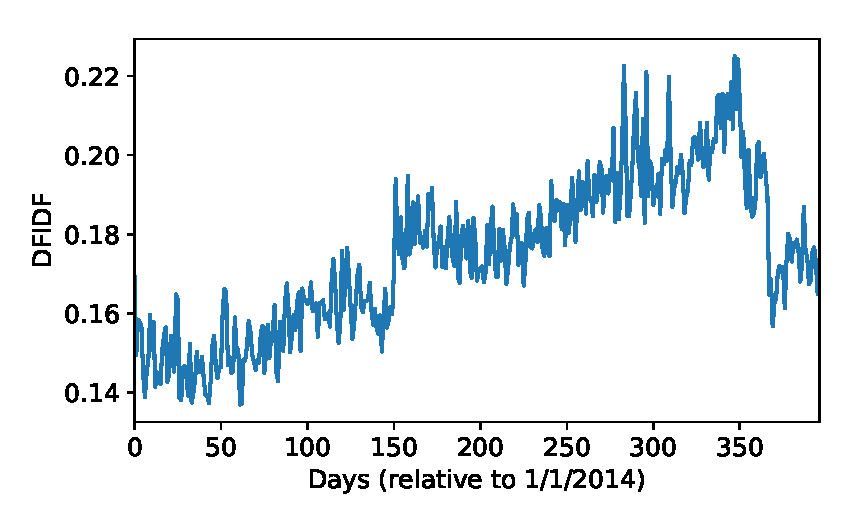
\includegraphics[width=\linewidth]{19_trajectory}  % noisy trajectory
  \caption{Event trajectory}
  \label{fig:noisy-trajectory}
\end{subfigure}%
\begin{subfigure}{.5\textwidth}
  \centering
  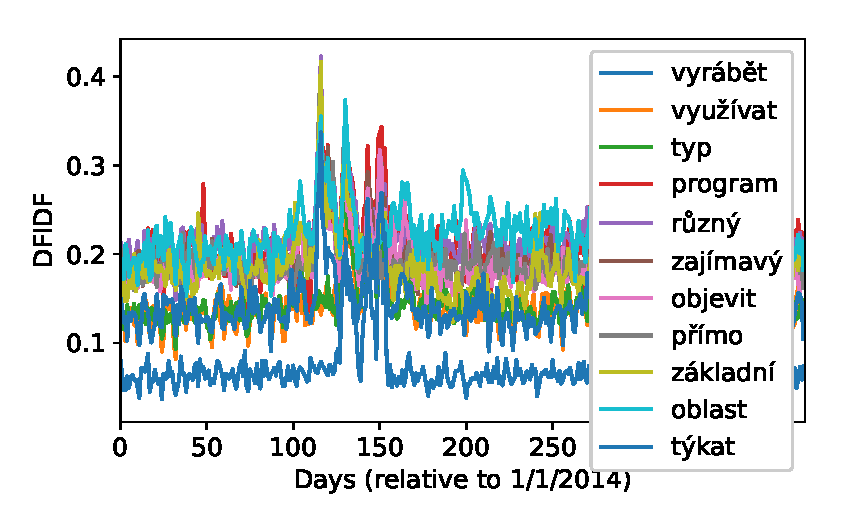
\includegraphics[width=\linewidth]{17_words}  % noisy keywords
  \caption{Event keywords}
  \label{fig:noisy-keywords}
\end{subfigure}
\caption{(a) Event with noisy trajectory. (b) Event with noisy keywords \textit{to make, to utilize, type, program, different, interesting, to discover, directly, basic, area, to concern}.}
\end{figure}


\hspace{\fill}

\begin{minipage}{\linewidth}
\centering
\begin{tabular}{ l c }\toprule[1.5pt]
\bf Method 	 & \bf Noisiness \\ \midrule
\bf Original &  50.94\% \\
\bf Greedy   &  37.80\% \\
\bf Cluster &  \bf 19.48\% \\ \bottomrule[1.25pt]
\end {tabular}\par
\captionof{table}{Noisiness comparison} \label{tab:title} 
\end{minipage}

\hspace{\fill}

Here, the cluster-based method performed the best, as the clustering algorithm chosen (DBSCAN) is capable of automatic filtering of noisy samples. With the distance function measuring both trajectory and keyword similarity, it filters out words unrelated to any event.

Poor performance of the original method is partially caused by its large redundancy. Even if a number of words with noisy trajectories appears in similar documents, the method would not group them together to a single event, but split into several noisy events. All of these noisy events then negatively contribute to the noisiness score.

Surprisingly, the greedy method did not perform the worst even though manual check revealed poor keyword quality {\color{red} TODO: As can be seen from the purity evaluation?}. This can again be explained by larger keyword sets of the greedy method, which makes even the noisy words clustered together into a smaller number of noisy events.

\newpage

\section{Purity}

All previous evaluations concerned the events on the keyword level. The purity measure will evaluate the event document sets in terms of topical consistency. This is a metric used by \cite{document-purity}.

The evaluation is similar to the standard measure of cluster purity in the sense that we measure the consistency of class labelling within each cluster. Each event is interpreted as a cluster of documents. Clearly, a high quality event should contain documents concerning similar topics. The problem is that our documents do not have any notion of class labels, which we will have to supplement.

We first assembled a list of 50 words from 1000 most often occurring Nouns and Verbs in document headlines. The words are \textit{Ukrajina (Ukraine), Rusko (Russia), policie (police), soud (court), Zeman, EU, Sparta, festival, Babiš, Putin, Google, ekonomika (economics), letadlo (airplane), východ (east), politika (politics), zabít (to kill), poslanec (deputy), armáda (army), Kyjev (Kiev), Škoda, hokejista (hockey player), fotbalista (football player), doprava (traffic), vražda (murder), Vánoce (Christmas), Francie (France), sport, NATO, Moskva (Moscow), ropa (petroleum), turnaj (tournament), Obama, referendum, ebola, parlament (parliament), koalice (coalition), Paříž (Paris), automobil, mistrovství (championship), elektrárna (power plant), Sýrie (Syria), islamista (islamist), Brusel (Brussels), olympiáda (olympics), sníh (snow), průmysl (industry), revoluce (revolution), výbuch (explosion), finance, terorista (terrorist)}. All documents that contained any of these words in their headline were tagged with the corresponding class label.

Then, for each event, we computed the fraction of documents with the most frequently appearing class label out of all tagged documents. The measure is a weighted average of these values across all events, with weights being the number of tagged documents within each event.

\hspace{\fill}

\begin{minipage}{\linewidth}
\centering
\begin{tabular}{ l c }\toprule[1.5pt]
\bf Method 	 & \bf Purity \\ \midrule
\bf Original &  30.53\% \\
\bf Greedy   &  {\color{red} TODO} \\
\bf Cluster &  \bf 61.08\% \\ \bottomrule[1.25pt]
\end {tabular}\par
\captionof{table}{Purity comparison} \label{tab:title} 
\end{minipage}

\hspace{\fill}

\section{Computation time}

Finally, we evaluate the computation time. We measure the execution time of the individual detection steps, so it is clear which parts are the bottlenecks. All experiments were performed on a laptop computer with a 64bit operating system, quad-core processor and 8GB RAM.

\hspace{\fill}

\begin{minipage}{\linewidth}
\centering
\begin{tabular}{ r c c c }\toprule[1.5pt]
\bf Unit & \bf Original & \bf Greedy & \bf Clusters \\ \midrule
Word2Vec embedding & --- & \multicolumn{2}{c}{3h 50min} \\
Bag of words model construction & \multicolumn{3}{c}{37min} \\
Word trajectories \& spectral analysis & \multicolumn{3}{c}{8s} \\
Event detection & 2min 12s & 50s & 4min 50s \\
Document retrieval & 7min 30s & {\color{red} TODO} & 7h 40min \\
Event annotation & {\color{red} TODO} & {\color{red} TODO} & {\color{red} TODO} \\ \midrule
\bf Total & & & \\ \bottomrule[1.25pt]

\end{tabular}\par
\captionof{table}{Computation time comparison} \label{tab:title}
\end{minipage}

\hspace{\fill}

{\color{red} TODO: Measure how much of the BOW model construction is taken by IO operations.}

{\color{red} TODO: Write a conclusion of this evaluation once the results are known.}

